\section{Introduction to Computer Vision}
\begin{frame}{}
    \LARGE Computer Vision: \textbf{Introduction}
\end{frame}

\begin{frame}{Computer Vision}
\centering
Building artificial systems that process, perceive, and reason about visual data
\end{frame}

\begin{frame}{Computer Vision is Everywhere}
\begin{figure}
\centering
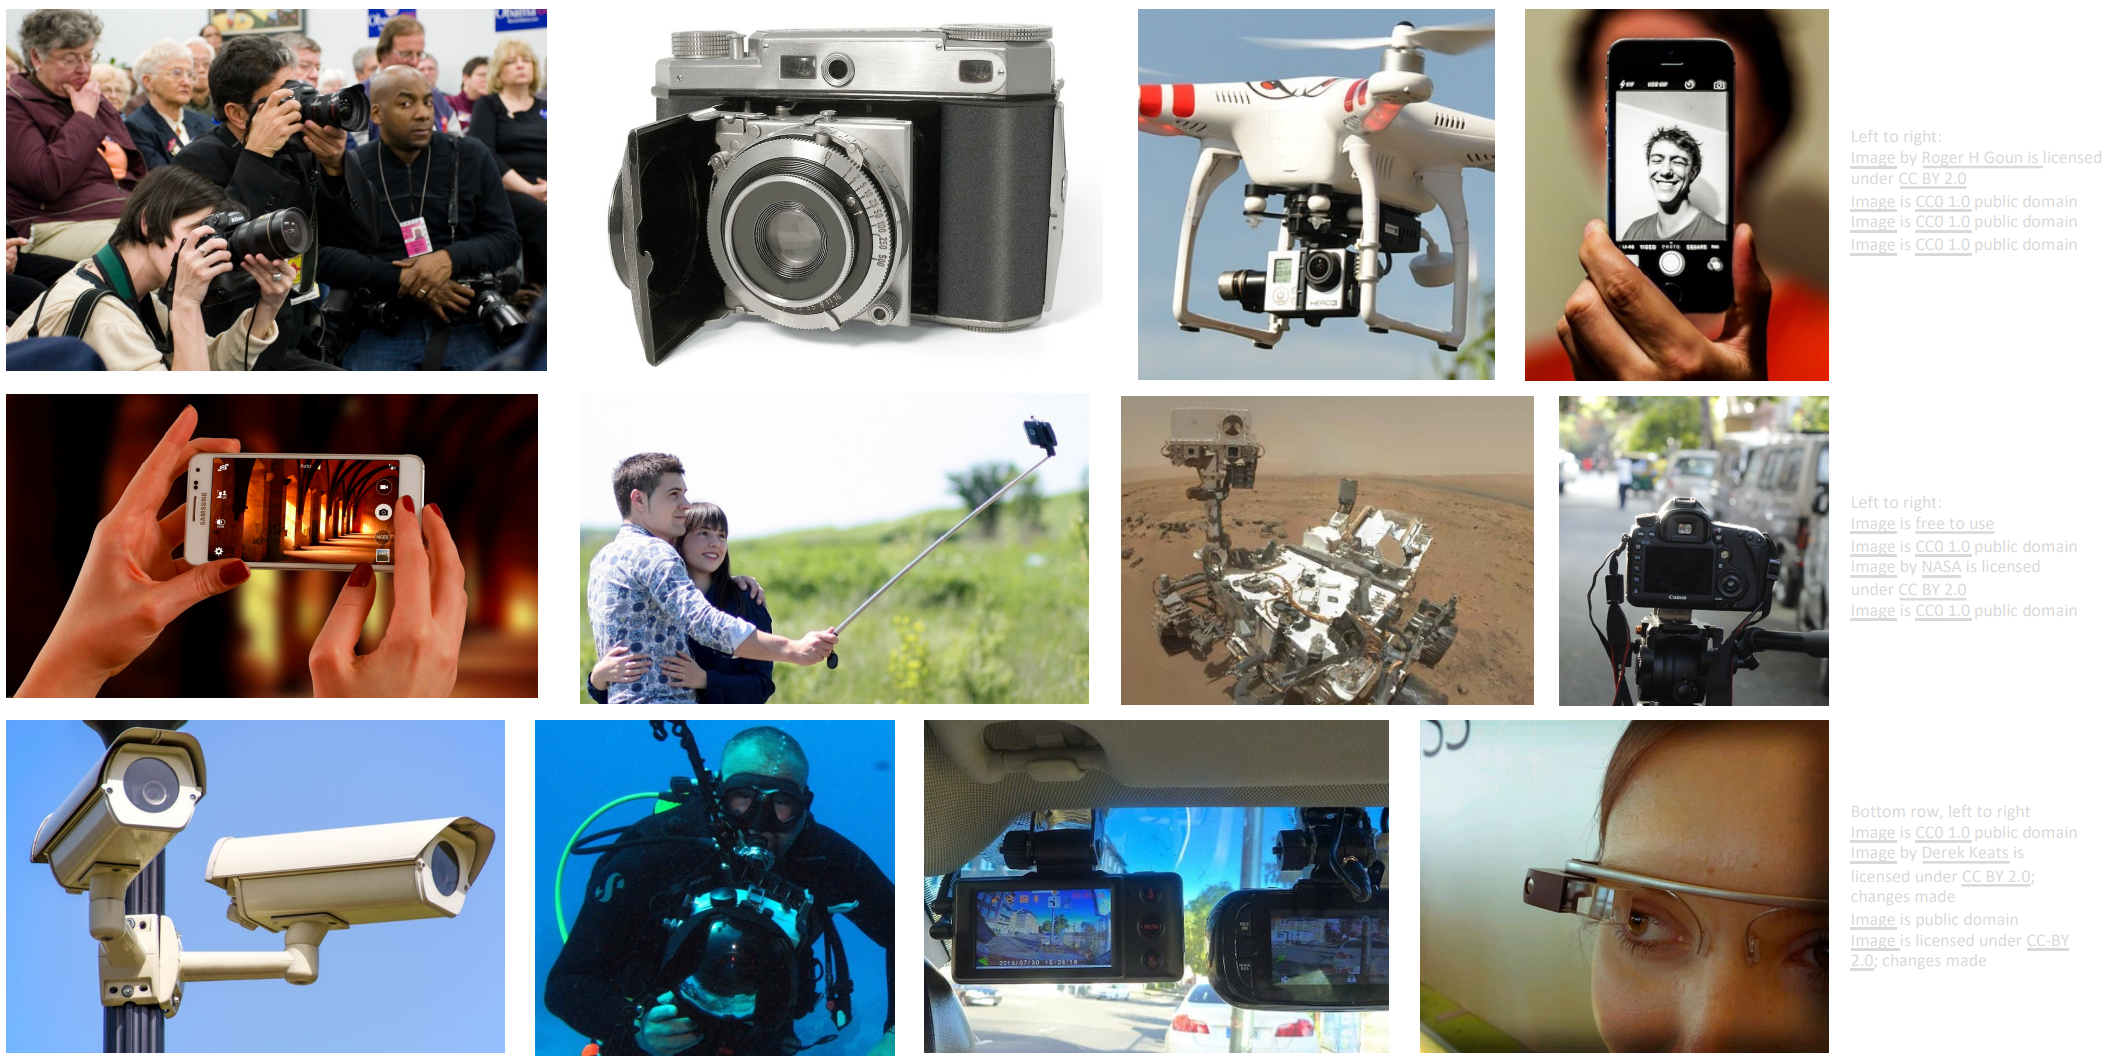
\includegraphics[width=1.0\textwidth,height=0.76\textheight,keepaspectratio]{images/cv-intro/cv_1.png}
\caption*{\scriptsize [Source: \url{https://machinelearningmastery.com/stanford-convolutional-neural-networks-for-visual-recognition-course-review/}]}
\end{figure}
\end{frame}

\begin{frame}[allowframebreaks]{Some Applications}
    \begin{figure}
        \centering
        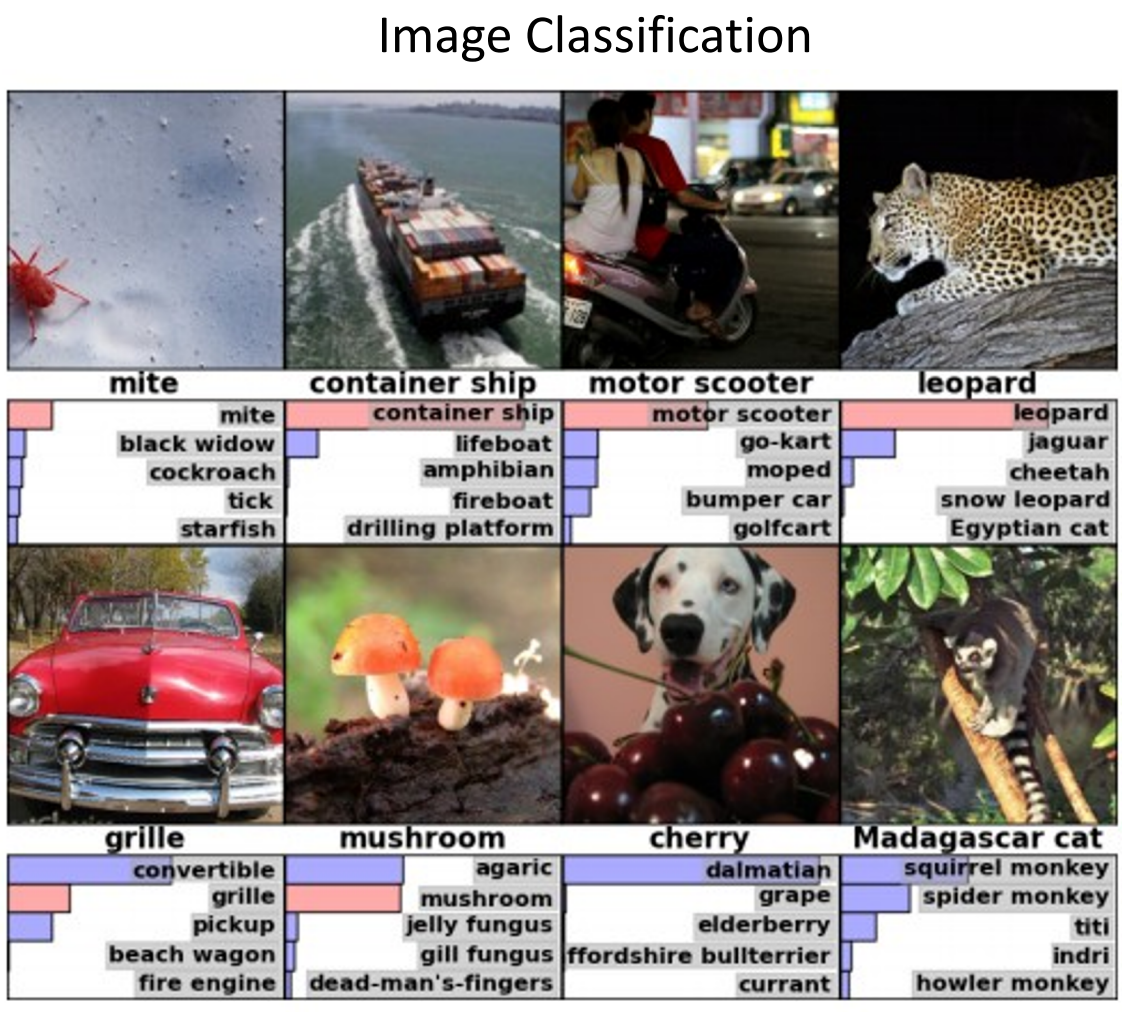
\includegraphics[height=0.8\textheight,width=1\textwidth,keepaspectratio]{images/cnn/cv_2.png}
        \caption*{\scriptsize Source: Krizhevsky, Sutskever \& Hinton, ``ImageNet Classification with Deep Convolutional Neural Networks'', NIPS 2012, Fig.~4 (left).}
    \end{figure}

    \framebreak

    \begin{figure}
        \centering
        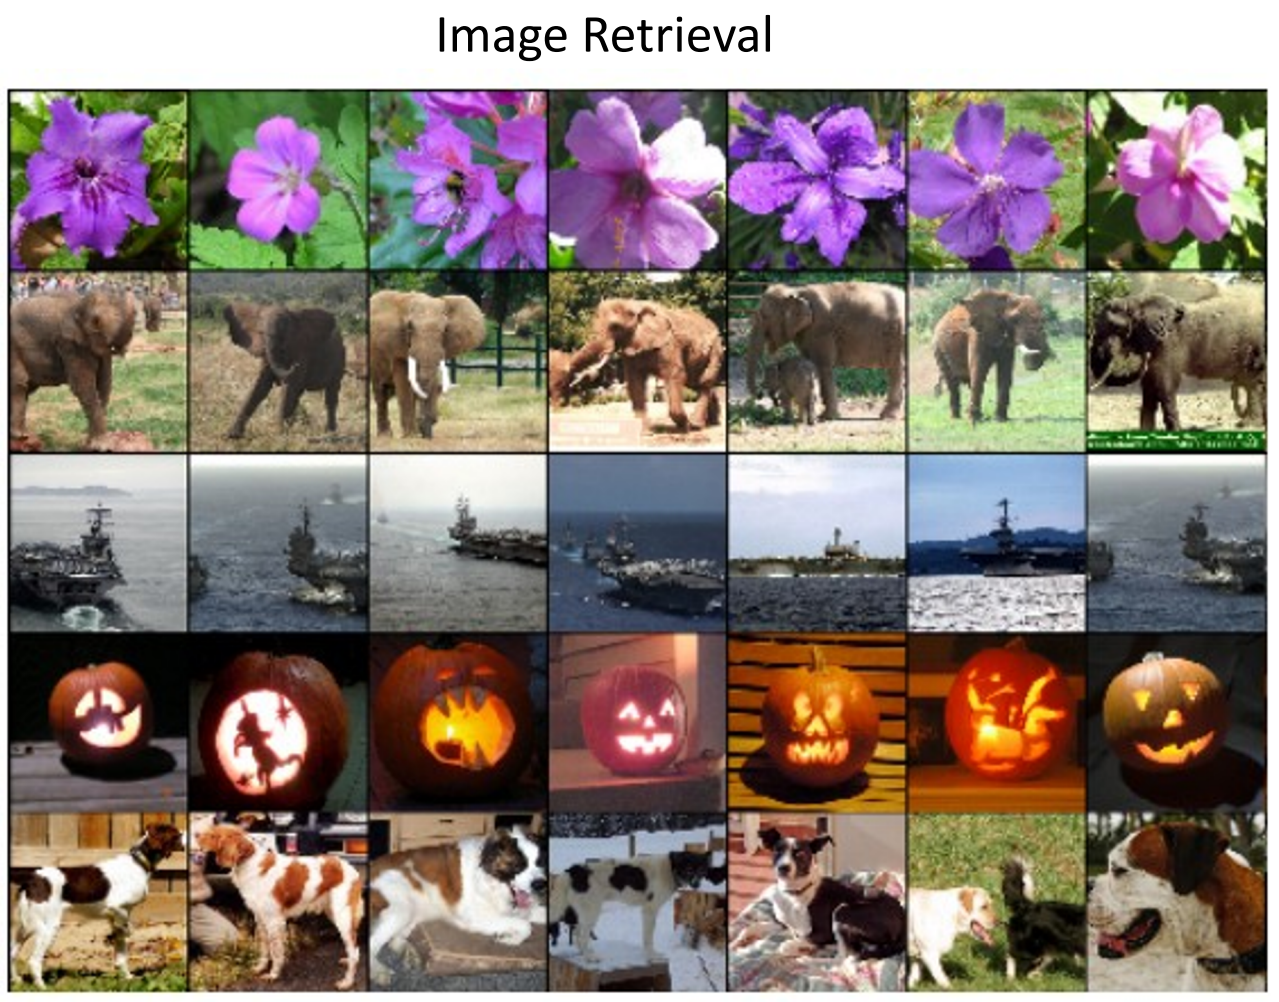
\includegraphics[height=0.8\textheight,width=1\textwidth,keepaspectratio]{images/cnn/cv_3.png}
        \caption*{\scriptsize Source: Krizhevsky, Sutskever \& Hinton, ``ImageNet Classification with Deep Convolutional Neural Networks'', NIPS 2012, Fig.~4 (right).}
    \end{figure}

    \framebreak

    % cv_4 -- cv_13 were previously emitted by a \foreach loop; unrolled so the
    % figures that carry no credit inside the bitmap can take their own caption.
    \begin{figure}
        \centering
        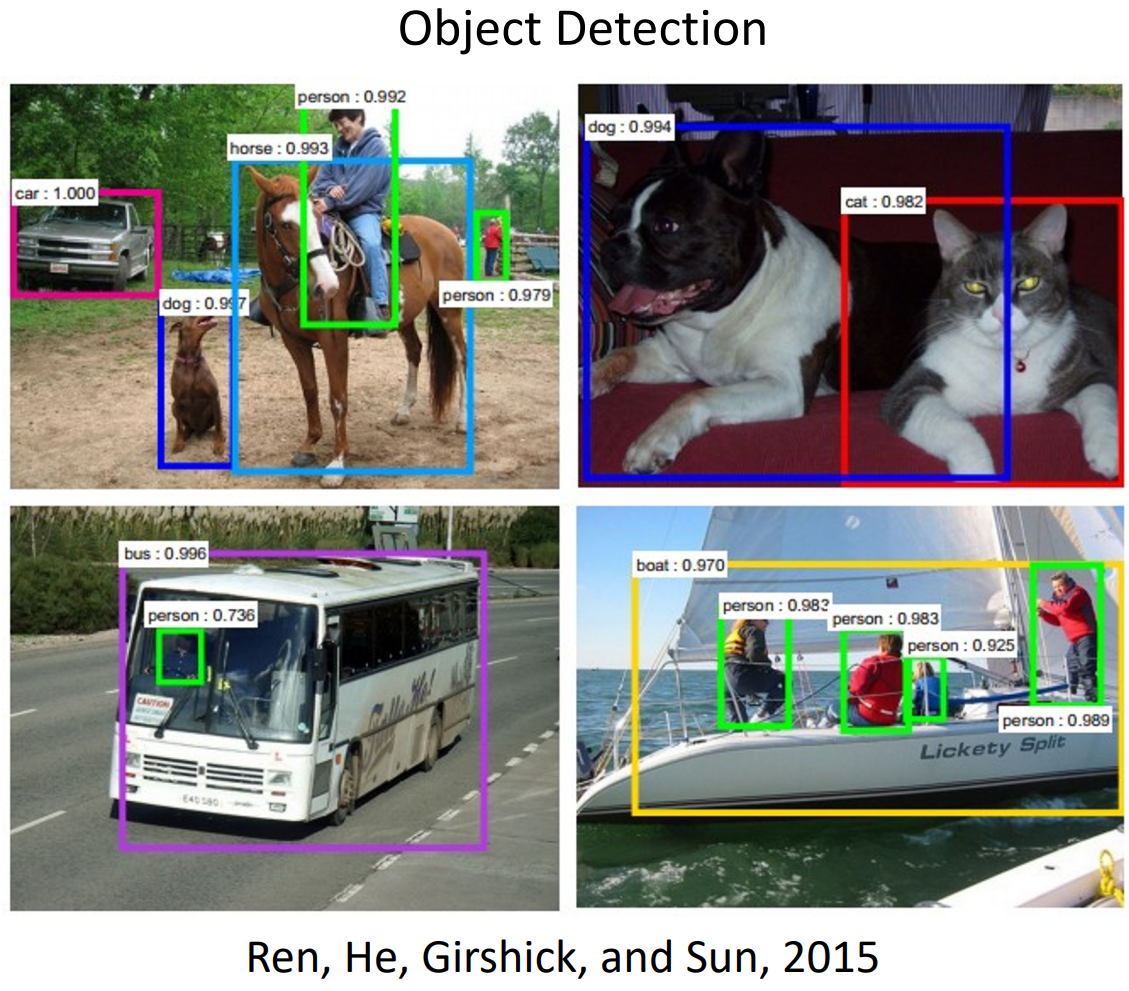
\includegraphics[height=0.9\textheight,width=1\textwidth,keepaspectratio]{images/cnn/cv_4.png}
    \end{figure}

    \framebreak

    \begin{figure}
        \centering
        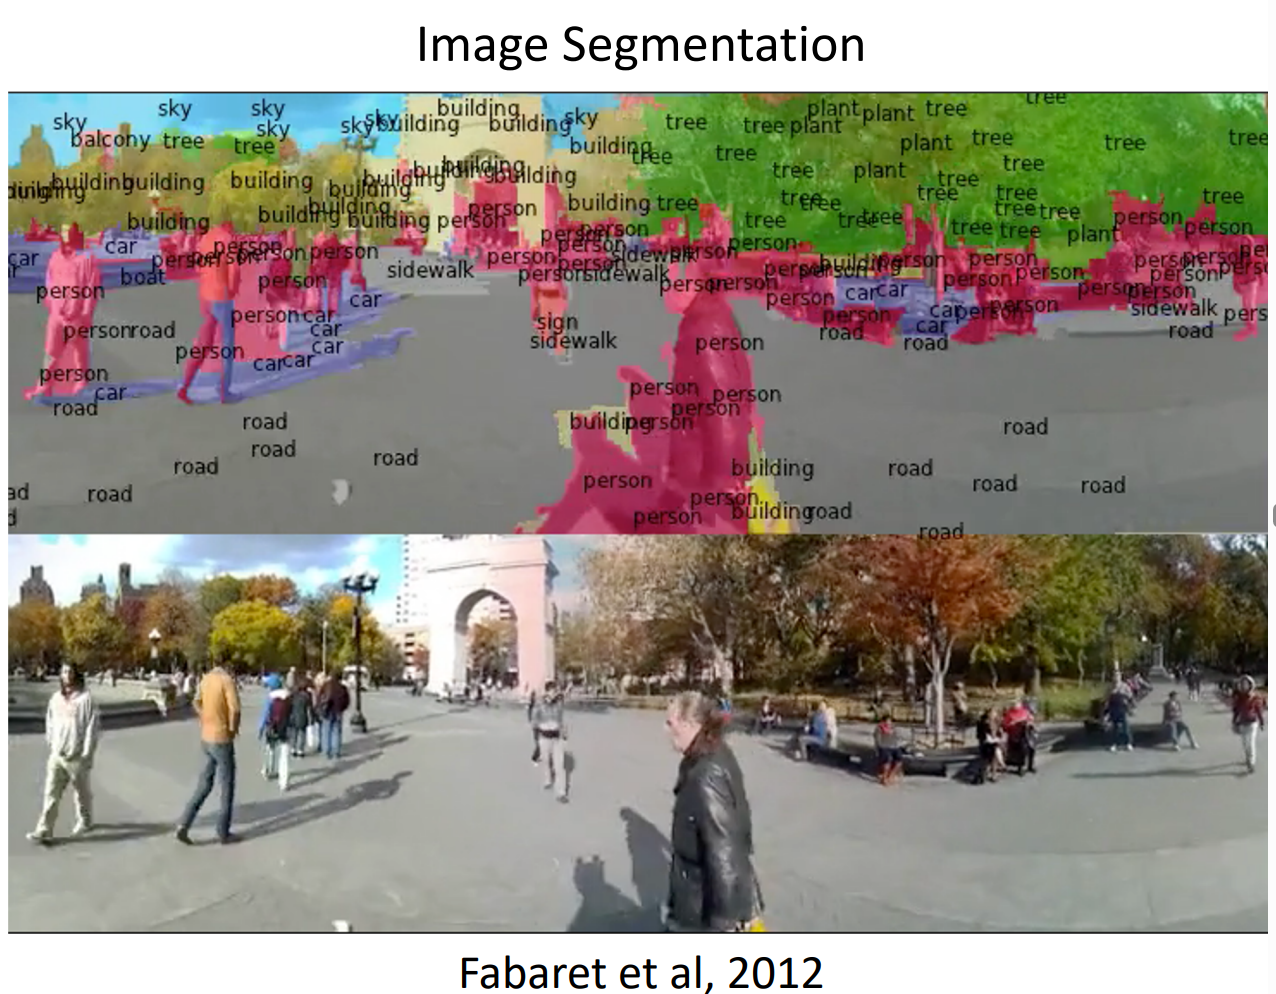
\includegraphics[height=0.9\textheight,width=1\textwidth,keepaspectratio]{images/cnn/cv_5.png}
    \end{figure}

    \framebreak

    \begin{figure}
        \centering
        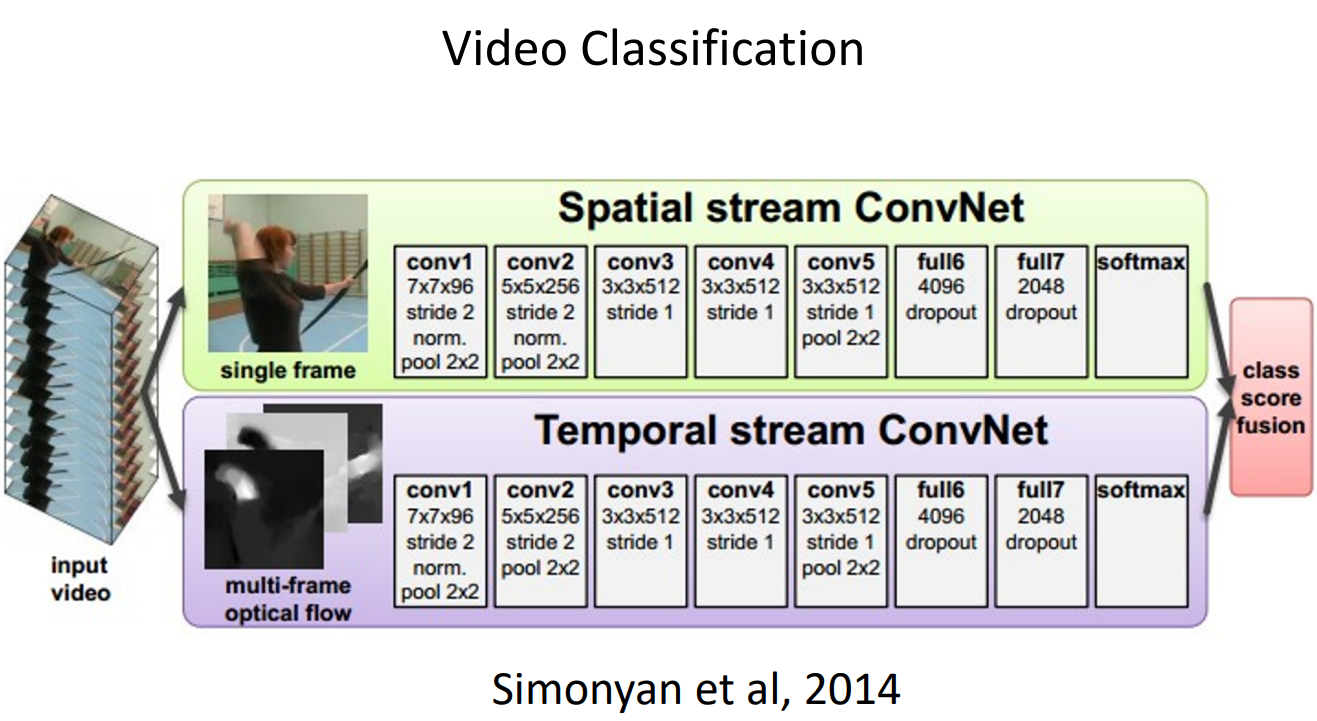
\includegraphics[height=0.9\textheight,width=1\textwidth,keepaspectratio]{images/cnn/cv_6.png}
    \end{figure}

    \framebreak

    \begin{figure}
        \centering
        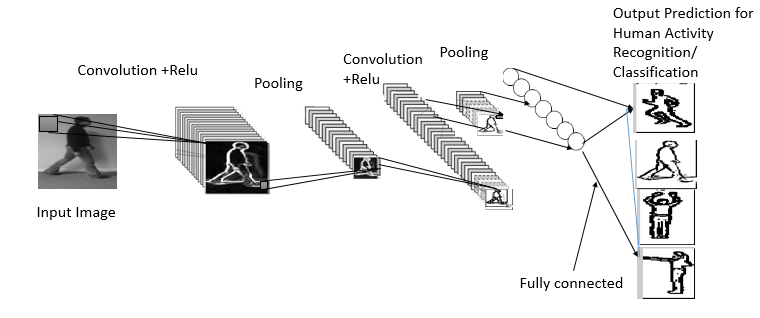
\includegraphics[height=0.8\textheight,width=1\textwidth,keepaspectratio]{images/cnn/cv_7.png}
        \caption*{\scriptsize [Source: \url{https://www.researchgate.net/figure/Convolutional-Neural-Network-Architecture-Design-for-Human-Activity-Recognition_fig1_330333654}]}
    \end{figure}

    \framebreak

    \begin{figure}
        \centering
        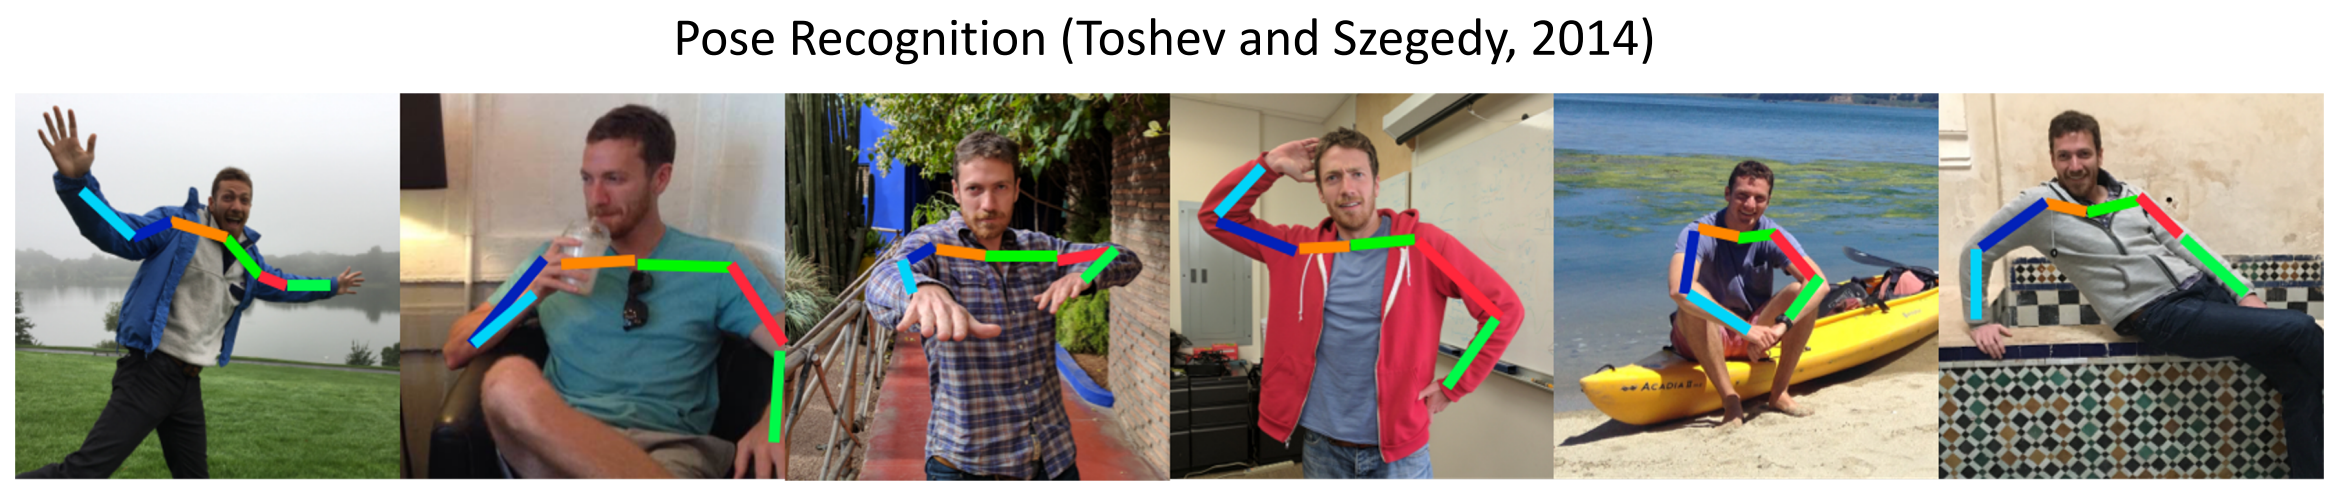
\includegraphics[height=0.9\textheight,width=1\textwidth,keepaspectratio]{images/cnn/cv_8.png}
    \end{figure}

    \framebreak

    \begin{figure}
        \centering
        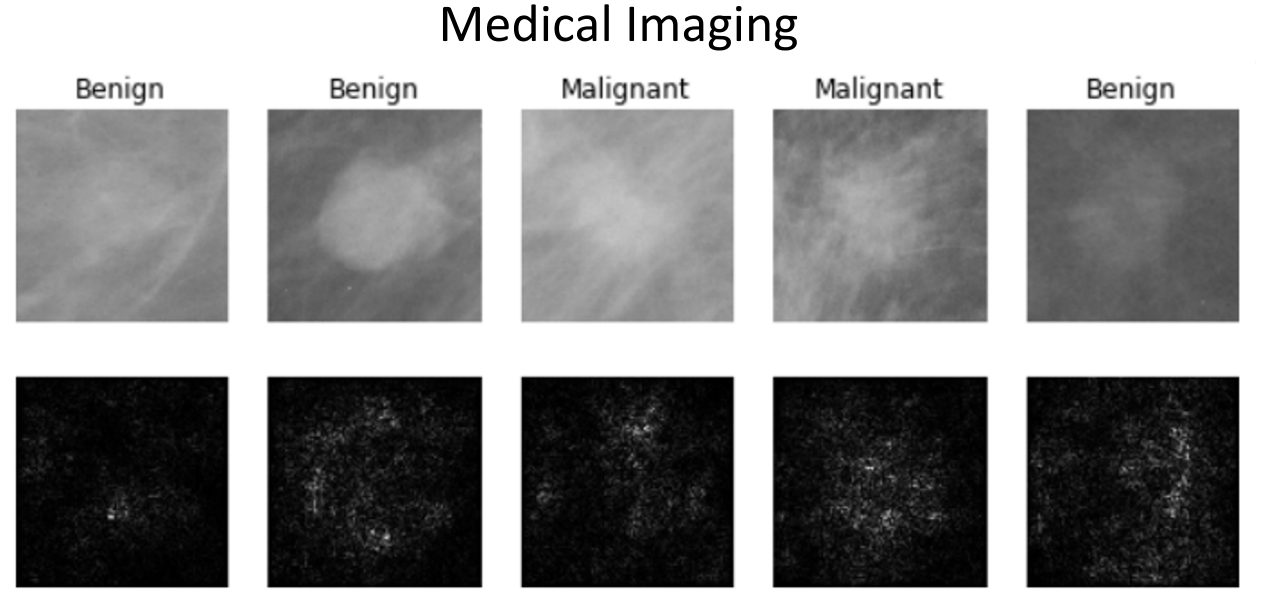
\includegraphics[height=0.8\textheight,width=1\textwidth,keepaspectratio]{images/cnn/cv_9.png}
        \caption*{\scriptsize [Source: \url{https://ai.stanford.edu/~danilevy/pdf/LevyJain16.pdf}]}
    \end{figure}

    \framebreak

    \begin{figure}
        \centering
        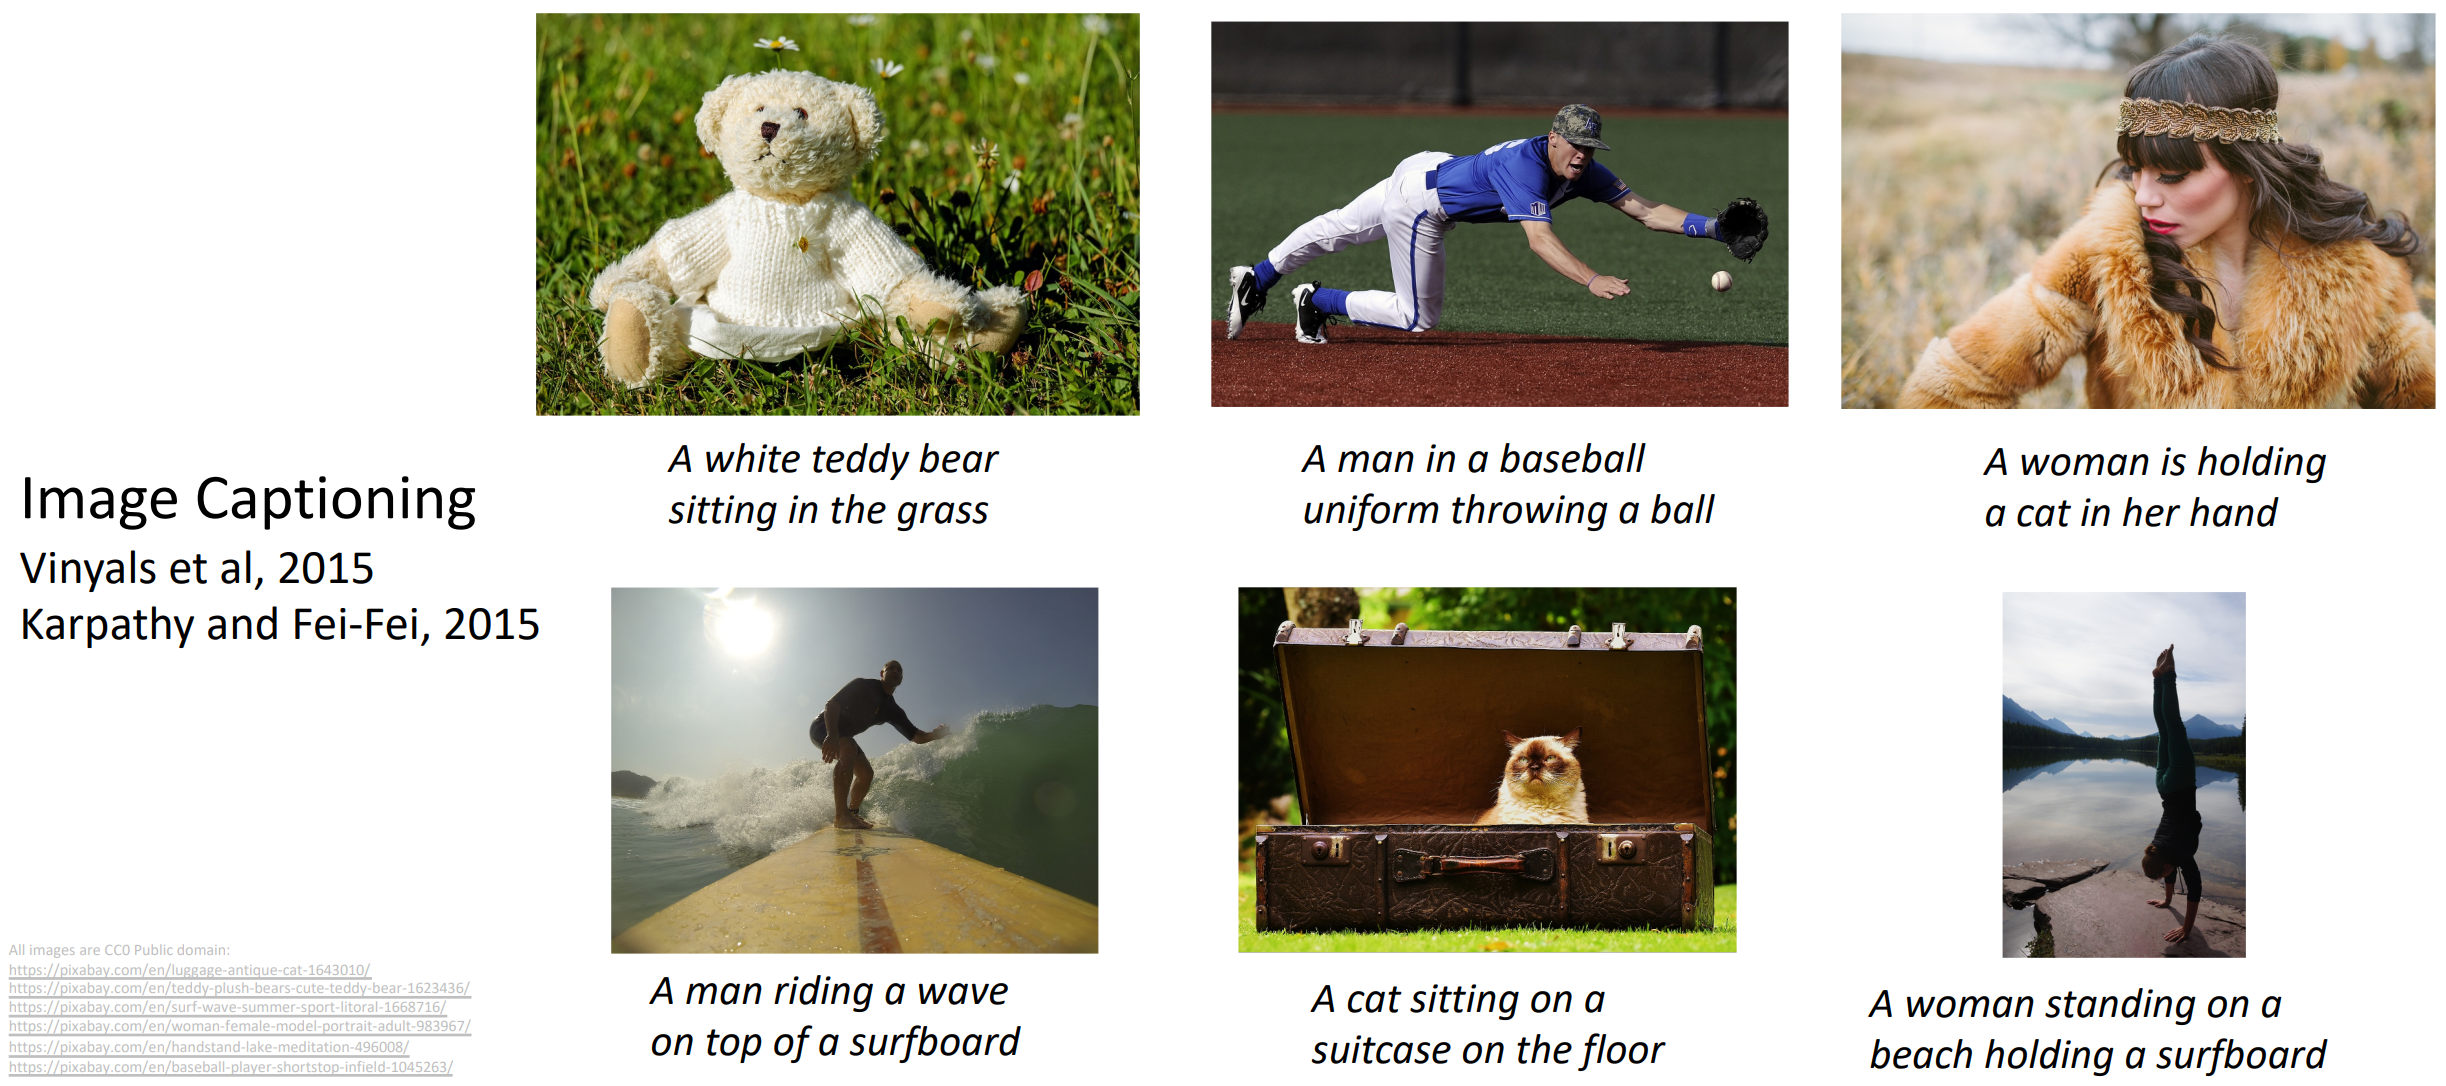
\includegraphics[height=0.9\textheight,width=1\textwidth,keepaspectratio]{images/cnn/cv_10.png}
    \end{figure}

    \framebreak

    \begin{figure}
        \centering
        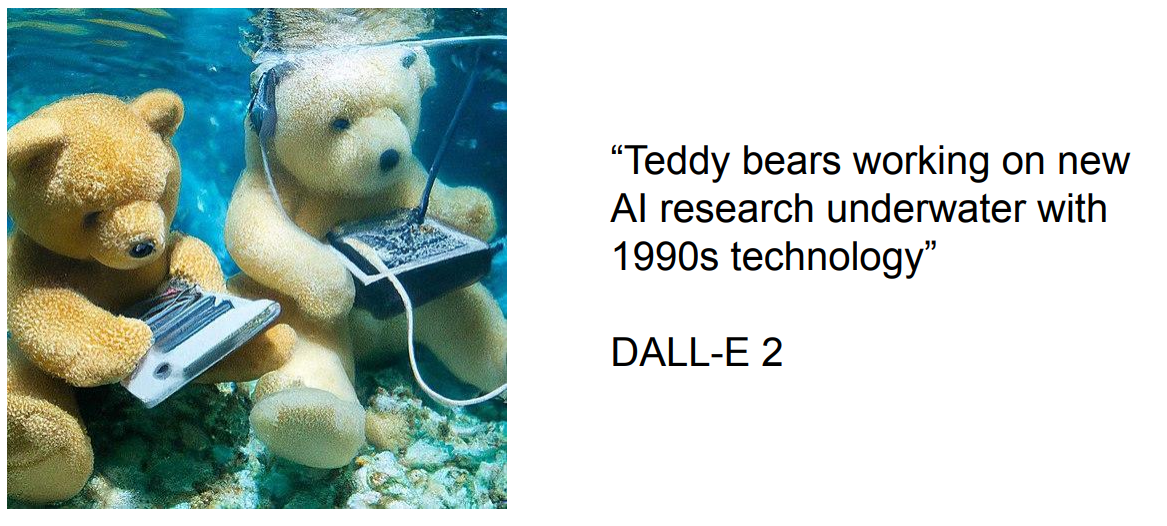
\includegraphics[height=0.9\textheight,width=1\textwidth,keepaspectratio]{images/cnn/cv_11.png}
    \end{figure}

    \framebreak

    \begin{figure}
        \centering
        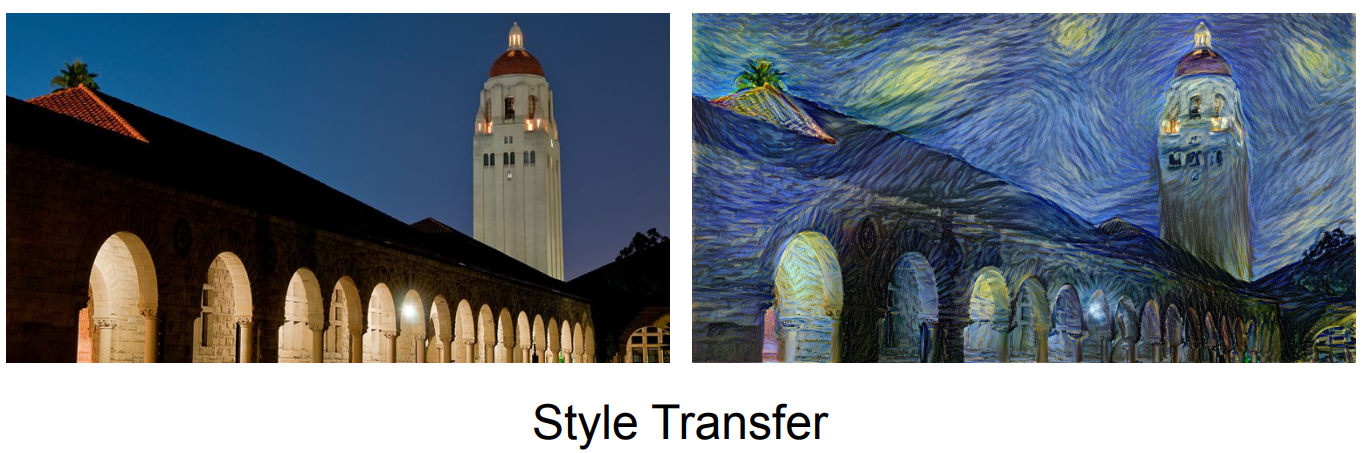
\includegraphics[height=0.8\textheight,width=1\textwidth,keepaspectratio]{images/cnn/cv_12.png}
        \caption*{\scriptsize [Source: \url{https://cs231n.stanford.edu/reports/2017/pdfs/401.pdf}]}
    \end{figure}

    \framebreak

    \begin{figure}
        \centering
        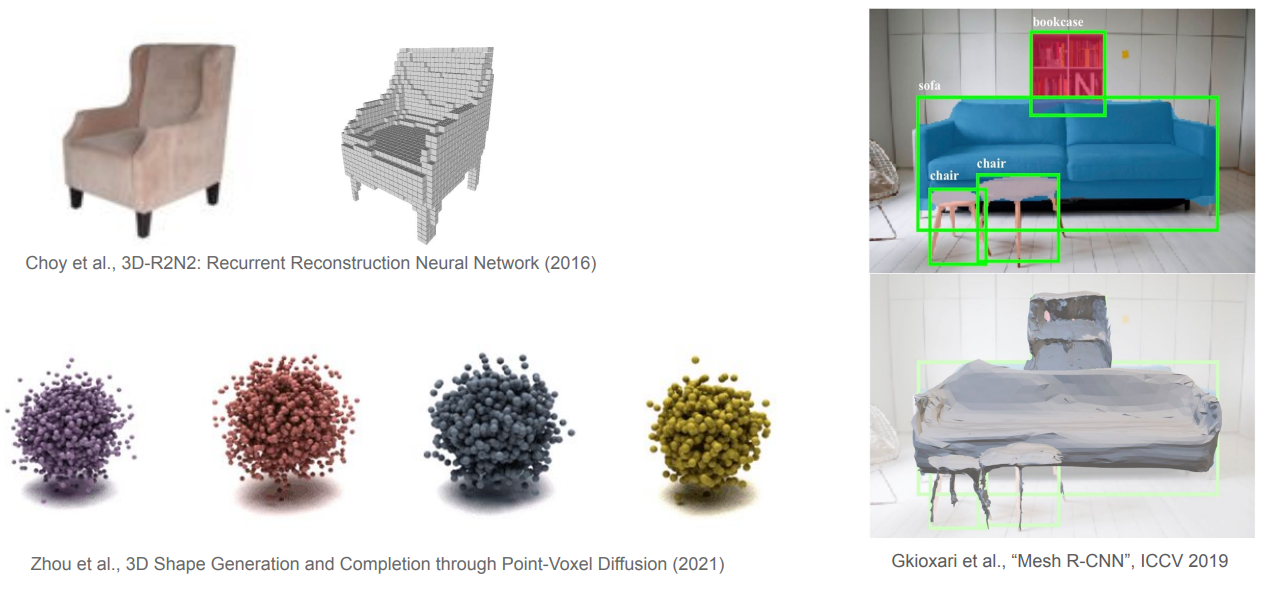
\includegraphics[height=0.9\textheight,width=1\textwidth,keepaspectratio]{images/cnn/cv_13.png}
    \end{figure}

    \framebreak
\end{frame}

\section{Image Representation}
\begin{frame}{How to represent an image?}
\begin{itemize}
    \item Images are represented as Matrices with elements in $[0,255]$
    \item Grayscale images have one channel.
\end{itemize}
\begin{figure}
\centering
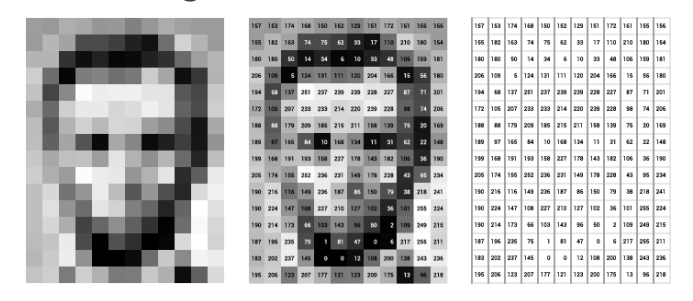
\includegraphics[width=1.0\textwidth,height=0.65\textheight,keepaspectratio]{images/cnn/represent_image.png}
\caption*{\scriptsize Source: V7 Labs, \textit{Image Recognition: Definition, Algorithms \& Uses}.}
\end{figure}
\end{frame}

\begin{frame}{How to represent an image?}
\begin{itemize}
    \item RGB images have 3 channels.
\end{itemize}
\begin{figure}
\centering
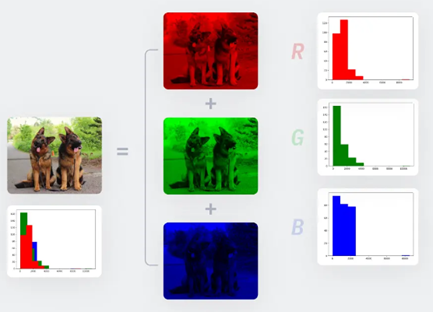
\includegraphics[width=1.5\textwidth,height=0.65\textheight,keepaspectratio]{images/cv-intro/RGB.png}
\caption*{\scriptsize [Source: \url{https://tech.ardswc.gov.tw/EPaper/Home/EPaper?PaperID=c57d55d5-109a-4319-816b-cc899e65f7a1}]}
\end{figure}
\end{frame}
